\documentclass[12pt]{article}

% =========================
% Toggle: show only problems, or problems + student solution boxes
% =========================
\newif\ifsolutions
\solutionstrue     % Use this for the student template with solution boxes.
%\solutionsfalse   % POF template: questions only.

% =========================
% Packages
% =========================
\usepackage[a4paper,margin=24mm]{geometry}
\usepackage{amsmath,amssymb,mathtools}
\usepackage{braket}
\usepackage{siunitx}
\usepackage[most]{tcolorbox}
\usepackage{enumitem}
\usepackage{graphicx}
\usepackage{xcolor}
\usepackage[T1]{fontenc}
\usepackage{lmodern}
\usepackage{microtype}
\usepackage{float} % Allows figure to be placed at exact desired location
\usepackage[hidelinks]{hyperref}

\sisetup{inter-unit-product = \ensuremath{{}\cdot{}}}
\renewcommand{\d}{\mathop{}\!\mathrm{d}}
\setlength{\parindent}{0pt}
\setlength{\parskip}{0.55em}
\setlist[enumerate,1]{label=(\alph*),itemsep=0.25em,topsep=0.25em}
\setlist[enumerate,2]{label=(\roman*),itemsep=0.15em,topsep=0.15em}

% =========================
% Boxes
% =========================
\tcbset{
  enhanced,
  breakable,
  boxrule=0.8pt,
  arc=1.5mm,
  left=2mm,right=2mm,top=1.5mm,bottom=1.5mm
}

\newtcolorbox{problembox}[1]{
  colback=gray!8,
  colframe=black,
  fonttitle=\bfseries,
  title={#1}
}

\newtcolorbox{solutionbox}{
  colback=blue!3,
  colframe=blue!60!black,
  title={Solution},
  fonttitle=\bfseries
}

\newtcolorbox{answerbox}{
  colback=yellow!10,
  colframe=orange!70!black,
  title={Final answer},
  fonttitle=\bfseries
}

\newtcolorbox{insightbox}{
  colback=green!5,
  colframe=green!50!black,
  title={Physical insight},
  fonttitle=\bfseries
}

\newcommand{\problemsep}{\vspace{0.8em}}

\newcommand{\placeholderfigure}[2][50mm]{%
	\begin{center}
		\fbox{\parbox[c][#1][c]{0.82\linewidth}{\centering\small Figure placeholder}}\\[0.3em]
		{\footnotesize\emph{Caption: #2}}
\end{center}}

\graphicspath{{figures/}}
\usepackage{fancyhdr}
\pagestyle{fancy}\fancyhf{}
\renewcommand{\headrulewidth}{0pt}
\fancyfoot[L]{\footnotesize Candidate 672128}
\fancyfoot[R]{\footnotesize Page \thepage\ of \pageref*{LastPage}}
\usepackage{lastpage}
\usepackage{array} % If you want to place figures in the folder 'figures' (cleaner)

\setcounter{secnumdepth}{0} % Avoids numbering of the section and subsection while allowing them to appear in the TOC



% ======================================================
% ======================================================
% ================                    ==================
% ================   BEGIN DOCUMENT   ==================
% ================                    ==================
% ======================================================
% ======================================================

\begin{document}

\begin{center}
	{\Large\bfseries QT01 -- Foundations of Quantum Mechanics\\[0.2em]
		Portfolio (POF) -- Week 8\\[0.3em]
		{\normalsize Weight: 70\% of module grade}\\[1em]
		Candidate number: 672128
	}
\end{center}


% ======================================================
% ======================================================
%                      Week 2
% ======================================================
% ======================================================
\section{Week 2}

% ======================================================
%                  Problem 1
% ======================================================
\begin{problembox}{Problem 1 \hfill [16 marks]}
At time $t=0$ a particle is represented by the wave function
\[
\psi(x,0)=
\begin{cases}
A\left(\dfrac{x}{a}\right), & 0\le x\le a,\\[0.8em]
A\dfrac{(b-x)}{(b-a)}, & a\le x\le b,\\[0.8em]
0, & \text{otherwise},
\end{cases}
\]
where $A$, $a$, and $b$ are positive real constants.

\begin{enumerate}
    \item Normalise $\psi$ (that is, find $A$, in terms of $a$ and $b$).
    \item Sketch $\psi(x,0)$, as a function of $x$.
    \item Where is the particle most likely to be found, at $t=0$?
    \item What is the probability of finding the particle to the left of $a$? Check your result in the limiting cases $b=a$ and $b=2a$.
    \item What is the expectation value of $x$?
\end{enumerate}
\end{problembox}

% ======================================================
%                  Solution 1
% ======================================================
\ifsolutions
\begin{solutionbox}
\textbf{Given.} A real, piecewise-linear wave function that rises from $0$ at $x=0$ to $A$ at $x=a$, falls back to $0$ at $x=b$, and vanishes elsewhere; $A,a,b>0$ with $b>a$. \textbf{Goal.} Fix $A$, locate the most probable position, find $P(x<a)$ and $\langle x\rangle$.

\textbf{Principle.} By the Born rule, $|\psi(x,0)|^2\,\d x$ is the probability of finding the particle in $[x,x+\d x]$. The total probability must be one, which fixes $A$; probabilities over a region and the mean position are then integrals of $|\psi|^2$ over that region. Because $\psi$ is real, $|\psi|^2=\psi^2$.

\textbf{(a) Normalisation.} Only $0\le x\le b$ contributes:
\begin{align*}
1=\int_{-\infty}^{\infty}|\psi|^2\,\d x
&=\frac{|A|^2}{a^2}\int_0^a x^2\,\d x+\frac{|A|^2}{(b-a)^2}\int_a^b (b-x)^2\,\d x\\
&=\frac{|A|^2}{a^2}\cdot\frac{a^3}{3}+\frac{|A|^2}{(b-a)^2}\cdot\frac{(b-a)^3}{3}
=|A|^2\left(\frac{a}{3}+\frac{b-a}{3}\right)=\frac{|A|^2\,b}{3}.
\end{align*}
(The second integral uses $u=b-x$, so $\int_a^b(b-x)^2\d x=\int_0^{b-a}u^2\d u$.) Choosing the overall phase so that $A$ is real and positive, $A=\sqrt{3/b}$.

\textbf{(b) Sketch.} $\psi$ is a triangle: zero outside $[0,b]$, a straight rise of slope $A/a$ to the apex $A$ at $x=a$, then a straight fall of slope $-A/(b-a)$ back to zero at $x=b$ (Figure~\ref{fig:tri}). It is continuous everywhere but has kinks at $x=0,a,b$.
\begin{figure}[H]
\centering
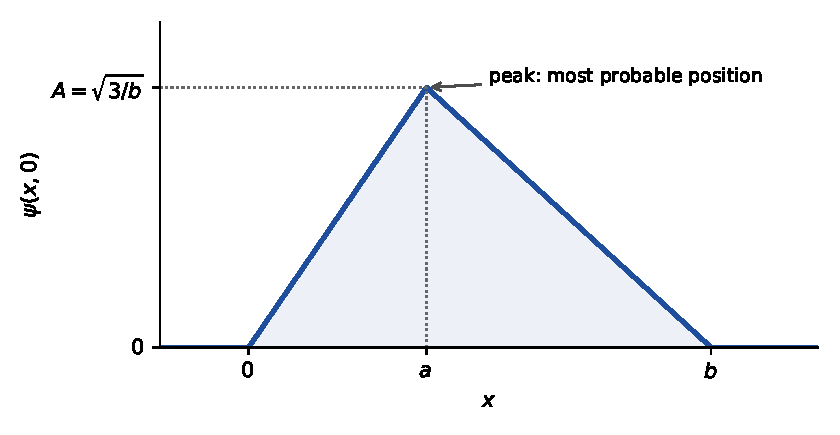
\includegraphics[width=0.78\linewidth]{psi_triangle}
\caption{$\psi(x,0)$ for the illustrative choice $b=2.6\,a$. The apex at $x=a$ has height $A=\sqrt{3/b}$.}
\label{fig:tri}
\end{figure}

\textbf{(c) Most probable position.} $|\psi|^2$ increases monotonically on $[0,a]$ (as $x^2$) and decreases monotonically on $[a,b]$ (as $(b-x)^2$), so its maximum is at the apex, $x=a$.

\textbf{(d) Probability to the left of $a$.}
\[
P(x<a)=\int_0^a|\psi|^2\,\d x=\frac{|A|^2}{a^2}\cdot\frac{a^3}{3}=\frac{3}{b}\cdot\frac{a}{3}=\frac{a}{b}.
\]
\emph{Limiting cases.} For $b\to 2a$: $P=\tfrac12$. The triangle is then symmetric about $x=a$, so the particle is equally likely to be found on either side, as it must be. For $b\to a$: $P\to 1$. The falling edge becomes vertical, the region $a<x<b$ shrinks to zero width and carries no probability, so the particle is certainly to the left of $a$. (At exactly $b=a$ the second line of $\psi$ is $0/0$ and undefined, so this case is understood as the limit $b\to a^+$; both wordings of the question give the same two checks.)

\textbf{(e) Expectation value of $x$.}
\[
\langle x\rangle=\int x|\psi|^2\,\d x
=\frac{|A|^2}{a^2}\int_0^a x^3\,\d x+\frac{|A|^2}{(b-a)^2}\int_a^b x(b-x)^2\,\d x .
\]
The first integral is $a^4/4$. In the second put $u=b-x$, $x=b-u$:
\[
\int_0^{b-a}(b-u)u^2\,\d u=\frac{b(b-a)^3}{3}-\frac{(b-a)^4}{4}.
\]
Hence, with $|A|^2=3/b$,
\begin{align*}
\langle x\rangle
&=\frac{3}{b}\left[\frac{a^2}{4}+\frac{b(b-a)}{3}-\frac{(b-a)^2}{4}\right]
=\frac{3}{b}\left[\frac{(2a-b)\,b}{4}+\frac{b(b-a)}{3}\right]\\
&=\frac{3(2a-b)}{4}+(b-a)=\frac{2a+b}{4},
\end{align*}
where $a^2-(b-a)^2=(2a-b)b$ was used.

\textbf{Checks.} Dimensions: $|A|^2=3/b$ has units of inverse length, as a 1D probability density requires; $P=a/b$ is dimensionless; $\langle x\rangle$ is a length. Range: $0<a/b<1$ is a valid probability for every $b>a$, and $0<\tfrac{2a+b}{4}<b$ (the second inequality is $2a<3b$), so the mean lies inside the region where $\psi\neq0$; it tends to $3a/4$ as $b\to a$ and equals $a$ for $b=2a$. Symmetry: for $b=2a$ the mean sits exactly at the apex $x=a$, consistent with (d). All four results were also confirmed by numerical quadrature for three different $(a,b)$ pairs.
\end{solutionbox}

\begin{answerbox}
\[
A=\sqrt{\frac{3}{b}},\qquad x_{\text{most probable}}=a,\qquad P(x<a)=\frac{a}{b},\qquad \langle x\rangle=\frac{2a+b}{4}.
\]
Therefore, the normalised state has $A=\sqrt{3/b}$, the particle is most likely to be found at the apex $x=a$, the probability of finding it to the left of $a$ is $a/b$ (which correctly gives $\tfrac12$ for $b=2a$ and $1$ for $b\to a$), and its mean position is $\langle x\rangle=(2a+b)/4$.
\end{answerbox}

\begin{insightbox}
The most probable position ($x=a$) and the mean position ($(2a+b)/4$) are different whenever the triangle is lopsided: for $b>2a$ the long tail to the right pulls the mean beyond the peak, just as a skewed classical distribution has mean $\neq$ mode. Only for the symmetric case $b=2a$ do they coincide. This is why ``where is the particle?'' has no single answer in quantum mechanics: the state specifies a whole distribution, and different questions (most likely value, average over many measurements) pick out different features of it.
\end{insightbox}
\fi

% ======================================================
%                  Problem 2
% ======================================================
\newpage
\begin{problembox}{Problem 2 \hfill [6 marks]}
In the concrete representation of bras and kets by row and column vectors, the inner product is defined in terms of components:
\[
\braket{B|A}
=
\begin{pmatrix}
\beta_1^* & \beta_2^* & \beta_3^*
\end{pmatrix}
\begin{pmatrix}
\alpha_1\\
\alpha_2\\
\alpha_3
\end{pmatrix}
=\beta_1^*\alpha_1+\beta_2^*\alpha_2+\beta_3^*\alpha_3.
\]

The rule for inner products is essentially the same as for dot products: add the products of corresponding components of the vectors whose inner product is being calculated.

Show that the inner product $\braket{B|A}$, defined as above, satisfies all the axioms of inner products (conjugate symmetry, linearity in the second argument, and positive-definiteness).
\end{problembox}

% ======================================================
%                  Solution 2
% ======================================================
\ifsolutions
\begin{solutionbox}
\textbf{Given.} $\ket{A}\leftrightarrow(\alpha_1,\alpha_2,\alpha_3)^{T}$, $\ket{B}\leftrightarrow(\beta_1,\beta_2,\beta_3)^{T}$ with complex components, and $\braket{B|A}=\sum_{i=1}^{3}\beta_i^*\alpha_i$. \textbf{Goal.} Verify the three inner-product axioms directly from this component formula, using only the arithmetic of complex numbers: $(z_1z_2)^*=z_1^*z_2^*$, $(z_1+z_2)^*=z_1^*+z_2^*$, $(z^*)^*=z$ and $z^*z=|z|^2\ge0$.

\textbf{1. Conjugate symmetry,} $\braket{B|A}=\braket{A|B}^*$. From the definition with the roles swapped, $\braket{A|B}=\sum_i\alpha_i^*\beta_i$. Taking the complex conjugate term by term,
\[
\braket{A|B}^*=\Big(\sum_i\alpha_i^*\beta_i\Big)^*=\sum_i(\alpha_i^*)^*\beta_i^*=\sum_i\beta_i^*\alpha_i=\braket{B|A}.
\]

\textbf{2. Linearity in the second argument.} Let $\ket{A}=c_1\ket{A_1}+c_2\ket{A_2}$ with $c_1,c_2\in\mathbb{C}$; its components are $\alpha_i=c_1\alpha_i^{(1)}+c_2\alpha_i^{(2)}$, because adding kets and multiplying by scalars act component by component on column vectors. Then
\[
\braket{B|A}=\sum_i\beta_i^*\big(c_1\alpha_i^{(1)}+c_2\alpha_i^{(2)}\big)
=c_1\sum_i\beta_i^*\alpha_i^{(1)}+c_2\sum_i\beta_i^*\alpha_i^{(2)}
=c_1\braket{B|A_1}+c_2\braket{B|A_2},
\]
using only the distributive law and the fact that the $c$'s are common to every term.

\textbf{3. Positive-definiteness.} Setting $\ket{B}=\ket{A}$,
\[
\braket{A|A}=\sum_i\alpha_i^*\alpha_i=|\alpha_1|^2+|\alpha_2|^2+|\alpha_3|^2 .
\]
Each term is a real, non-negative number, so $\braket{A|A}$ is real and $\braket{A|A}\ge0$. A sum of non-negative terms vanishes only if every term vanishes, so $\braket{A|A}=0\iff\alpha_1=\alpha_2=\alpha_3=0\iff\ket{A}=\mathbf 0$.

\textbf{Consequence (check).} Combining 1 and 2 gives \emph{antilinearity in the first argument}: for $\ket{B}=d_1\ket{B_1}+d_2\ket{B_2}$, $\braket{B|A}=\braket{A|B}^*=(d_1\braket{A|B_1}+d_2\braket{A|B_2})^*=d_1^*\braket{B_1|A}+d_2^*\braket{B_2|A}$, which is exactly what the explicit $\beta_i^*$ in the definition produces. This consistency confirms that the complex conjugate on the bra side is essential: without it, $\braket{A|A}=\sum_i\alpha_i^2$ could be negative or complex (e.g.\ $\alpha=(i,0,0)$ gives $-1$). All three properties were also checked numerically on 1000 random complex vectors.
\end{solutionbox}

\begin{answerbox}
For all $\ket{A},\ket{B}\in\mathbb{C}^3$ and $c_1,c_2\in\mathbb{C}$:
\begin{gather*}
\braket{B|A}=\braket{A|B}^*,\qquad
\braket{B|c_1A_1+c_2A_2}=c_1\braket{B|A_1}+c_2\braket{B|A_2},\\
\braket{A|A}=\textstyle\sum_i|\alpha_i|^2\ge0\quad(=0\iff\ket{A}=0).
\end{gather*}
Therefore, the component rule $\braket{B|A}=\sum_i\beta_i^*\alpha_i$ satisfies conjugate symmetry, linearity in the second argument and positive-definiteness, so it is a genuine inner product on $\mathbb{C}^3$.
\end{answerbox}

\begin{insightbox}
Positive-definiteness is what lets $\braket{A|A}$ act as a squared length, and hence what makes normalisation $\braket{\psi|\psi}=1$ and the Born-rule probabilities $|\braket{\phi_n|\psi}|^2$ meaningful. The complex conjugation that distinguishes this from an ordinary dot product is the price of working with complex amplitudes: it is exactly what guarantees that ``lengths'' and probabilities come out real and non-negative.
\end{insightbox}
\fi


\newpage
% ======================================================
% ======================================================
%                      Week 3
% ======================================================
% ======================================================
\section{Week 3}

% ======================================================
%                  Problem 1
% ======================================================
\begin{problembox}{Problem 1 \hfill [12 marks]}
Show that the position operator 
\[
\hat{x}=x,
\]
and momentum operator
\[
\hat{p}=\frac{\hbar}{i}\frac{\partial}{\partial x},
\]
are Hermitian, in other words, that
\[
\braket{\phi|\hat{x}\psi}=\braket{\hat{x}\phi|\psi}
\qquad\text{and}\qquad
\braket{\phi|\hat{p}\psi}=\braket{\hat{p}\phi|\psi}.
\]
\end{problembox}

% ======================================================
%                  Solution 1
% ======================================================
\ifsolutions
\begin{solutionbox}
\textbf{Given.} $\hat x=x$ (multiplication by $x$) and $\hat p=\frac{\hbar}{i}\frac{\partial}{\partial x}$, acting on wave functions in one dimension, with $\braket{f|g}=\int_{-\infty}^{\infty}f^*(x)\,g(x)\,\d x$. \textbf{Goal.} Show $\braket{\phi|\hat x\psi}=\braket{\hat x\phi|\psi}$ and $\braket{\phi|\hat p\psi}=\braket{\hat p\phi|\psi}$ for all physically admissible $\phi,\psi$.

\textbf{Assumption.} $\phi$ and $\psi$ are square-integrable (normalisable) states, so $\phi,\psi\to0$ as $|x|\to\infty$; this is the condition every physical state satisfies, and it is what makes the boundary terms below vanish.

\textbf{Position operator.} Because $x$ is a real number at every point, $x^*=x$, so
\[
\braket{\phi|\hat x\psi}=\int\phi^*(x)\,x\,\psi(x)\,\d x=\int\big(x\,\phi(x)\big)^*\psi(x)\,\d x=\braket{\hat x\phi|\psi}.
\]
Hence $\hat x$ is Hermitian. The same one-line argument applies to multiplication by any real function, e.g.\ a potential $V(x)$.

\textbf{Momentum operator.} Write the left-hand side and integrate by parts, with $u=\phi^*$ and $\d v=\frac{\partial\psi}{\partial x}\d x$:
\begin{align*}
\braket{\phi|\hat p\psi}
&=\int_{-\infty}^{\infty}\phi^*\,\frac{\hbar}{i}\frac{\partial\psi}{\partial x}\,\d x
=\frac{\hbar}{i}\Big[\phi^*\psi\Big]_{-\infty}^{\infty}-\frac{\hbar}{i}\int_{-\infty}^{\infty}\frac{\partial\phi^*}{\partial x}\,\psi\,\d x .
\end{align*}
The boundary term is zero because both functions vanish at $\pm\infty$. For the remaining term, note that $\frac{\hbar}{i}=-i\hbar$, so $-\frac{\hbar}{i}=i\hbar=\big(\frac{\hbar}{i}\big)^*$, and $\frac{\partial\phi^*}{\partial x}=\big(\frac{\partial\phi}{\partial x}\big)^*$. Therefore
\[
\braket{\phi|\hat p\psi}=\int_{-\infty}^{\infty}\Big(\frac{\hbar}{i}\frac{\partial\phi}{\partial x}\Big)^*\psi\,\d x=\braket{\hat p\phi|\psi}.
\]
Hence $\hat p$ is Hermitian.

\textbf{Why the factor $i$ matters (check).} Integration by parts alone produced a \emph{minus} sign: the bare derivative satisfies $\braket{\phi|\partial_x\psi}=-\braket{\partial_x\phi|\psi}$, i.e.\ $\partial_x$ is anti-Hermitian. The complex conjugation of $1/i$ supplies a second minus sign that cancels it, which is exactly why momentum carries a factor of $i$. Both identities, and the anti-Hermiticity of $\partial_x$ on its own, were confirmed numerically by quadrature with finite-difference derivatives on two arbitrary complex, normalisable test functions.
\end{solutionbox}

\begin{answerbox}
\[
\braket{\phi|\hat x\psi}=\braket{\hat x\phi|\psi},\qquad
\braket{\phi|\hat p\psi}=\braket{\hat p\phi|\psi}\quad\text{for all normalisable }\phi,\psi .
\]
Therefore, both $\hat x$ and $\hat p$ are Hermitian: $\hat x$ because $x$ is real, and $\hat p$ because the minus sign from integrating by parts (with vanishing boundary terms) is cancelled by the complex conjugate of the factor $\hbar/i$.
\end{answerbox}

\begin{insightbox}
Hermiticity is what makes $\hat x$ and $\hat p$ legitimate observables: it guarantees real expectation values ($\braket{\psi|\hat p\psi}=\braket{\hat p\psi|\psi}=\braket{\psi|\hat p\psi}^*$) and real eigenvalues, as any measured position or momentum must be. The proof also shows that Hermiticity of $\hat p$ depends on the space of states, through the boundary term: it is the normalisability of physical wave functions that makes momentum an observable.
\end{insightbox}
\fi

% ======================================================
%                  Problem 2
% ======================================================
\newpage
\begin{problembox}{Problem 2 \hfill [8 marks]}
The wave function of an electron in the lowest energy state of a hydrogen atom is proportional to $e^{-r/a_0}$, with $a_0$ a constant and $r$ the distance from the nucleus. Calculate the relative probabilities of finding the electron inside a region of volume $1.0\,\mathrm{pm}^3$, located at
\begin{itemize}
    \item the nucleus,
    \item a distance $a_0$ from the nucleus.
\end{itemize}

As the region of interest is so small, even on the scale of the atom, we can ignore the variation of $\psi$ within it.
\end{problembox}

% ======================================================
%                  Solution 2
% ======================================================
\ifsolutions
\begin{solutionbox}
\textbf{Given.} Hydrogen ground state $\psi(r)=N e^{-r/a_0}$; a small region of volume $\delta V=1.0\,\mathrm{pm}^3$ centred (i) at the nucleus, $r=0$, and (ii) at $r=a_0$. \textbf{Goal.} The ratio of the probabilities of finding the electron in the two regions.

\textbf{Principle.} By the Born rule in three dimensions, $|\psi(\mathbf r)|^2$ is a probability \emph{per unit volume}. The problem states that the region is so small that $\psi$ hardly varies across it, so the probability is the density at its centre times its volume:
\[
P\approx|\psi(\mathbf r)|^2\,\delta V .
\]

\textbf{Relative probability.} The normalisation constant $N$ and the common volume $\delta V$ cancel in the ratio, so $N$ is not needed:
\[
\frac{P(r=0)}{P(r=a_0)}=\frac{|N|^2e^{0}\,\delta V}{|N|^2e^{-2a_0/a_0}\,\delta V}=e^{2}\approx7.39 .
\]

\textbf{Absolute values (for scale).} Normalising, $\int_0^\infty|N|^2e^{-2r/a_0}\,4\pi r^2\,\d r=|N|^2\pi a_0^3=1$, so $|N|^2=1/(\pi a_0^3)$. With $a_0=52.9\,\mathrm{pm}$, $a_0^3=1.481\times10^{5}\,\mathrm{pm}^3$ and
\begin{align*}
P(r=0)&=\frac{\delta V}{\pi a_0^3}=\frac{1.0}{\pi\times1.481\times10^{5}}=2.15\times10^{-6},\\
P(r=a_0)&=P(r=0)\,e^{-2}=2.91\times10^{-7}.
\end{align*}

\textbf{Checks.} Both probabilities are dimensionless and far below 1, as they should be for a region of volume $\sim10^{-5}$ of the atom's $\sim a_0^3$. The ratio $2.15\times10^{-6}/2.91\times10^{-7}=7.39$ reproduces $e^2$. Testing the stated approximation numerically, averaging $|\psi|^2$ over an actual $1\,\mathrm{pm}$ cube gives a ratio of $7.26$, within $2\%$ of $e^2$: the approximation is good, and slightly generous at the nucleus because $e^{-r/a_0}$ has a cusp there.
\end{solutionbox}

\begin{answerbox}
\begin{gather*}
\frac{P(\text{nucleus})}{P(r=a_0)}=e^{2}\approx7.4,\\
P(\text{nucleus})\approx2.2\times10^{-6},\qquad P(r=a_0)\approx2.9\times10^{-7}\qquad(\delta V=1.0\,\mathrm{pm}^3).
\end{gather*}
Therefore, the electron is $e^2\approx7.4$ times more likely to be found in a $1\,\mathrm{pm}^3$ region at the nucleus than in an identical region a distance $a_0$ away, with absolute probabilities of about $2.2\times10^{-6}$ and $2.9\times10^{-7}$ respectively.
\end{answerbox}

\begin{insightbox}
This does not contradict the familiar statement that the electron is ``most likely found at $r=a_0$''. That statement concerns the \emph{radial} probability $P(r)\,\d r=4\pi r^2|\psi|^2\,\d r$, the probability of lying in a thin \emph{shell} of radius $r$; the shell's volume $4\pi r^2\d r$ grows from zero, and the product peaks at $r=a_0$. Per unit volume, by contrast, the density is greatest at the nucleus. The distinction between a probability density and the probability of a region is essential whenever results are quoted in three dimensions.
\end{insightbox}
\fi


\newpage
% ======================================================
% ======================================================
%                      Week 4
% ======================================================
% ======================================================
\section{Week 4}

% ======================================================
%                  Problem 1
% ======================================================
\begin{problembox}{Problem 1 \hfill [5 marks]}
Consider a system whose state is given in terms of an orthonormal set of three vectors: $\ket{\phi_1}$, $\ket{\phi_2}$, $\ket{\phi_3}$ as
\[
\ket{\psi}=\frac{\sqrt{3}}{3}\ket{\phi_1}+\frac{2}{3}\ket{\phi_2}+\frac{\sqrt{2}}{3}\ket{\phi_3}.
\]

\begin{enumerate}
    \item Verify that $\ket{\psi}$ is normalised. Then, calculate the probability of finding the system in any one of the states $\ket{\phi_1}$, $\ket{\phi_2}$ and $\ket{\phi_3}$. Verify that the total probability is equal to one.
    \item Consider now an ensemble of 810 identical systems, each one of them in the state $\psi$. If measurements are done on all of them, how many systems will be found in each of the states $\ket{\phi_1}$, $\ket{\phi_2}$ and $\ket{\phi_3}$?
\end{enumerate}
\end{problembox}

% ======================================================
%                  Solution 1
% ======================================================
\ifsolutions
\begin{solutionbox}
\textbf{Given.} $\ket{\psi}=c_1\ket{\phi_1}+c_2\ket{\phi_2}+c_3\ket{\phi_3}$ with $c_1=\frac{\sqrt3}{3}$, $c_2=\frac23$, $c_3=\frac{\sqrt2}{3}$, and $\braket{\phi_i|\phi_j}=\delta_{ij}$.

\textbf{Principle.} Because the basis is orthonormal, $\braket{\psi|\psi}=\sum_i|c_i|^2$ and $c_i=\braket{\phi_i|\psi}$. By the Born rule, a normalised state is found in $\ket{\phi_i}$ with probability $P_i=|\braket{\phi_i|\psi}|^2=|c_i|^2$.

\textbf{(a)} Normalisation:
\[
\braket{\psi|\psi}=\Big(\frac{\sqrt3}{3}\Big)^2+\Big(\frac23\Big)^2+\Big(\frac{\sqrt2}{3}\Big)^2=\frac39+\frac49+\frac29=\frac99=1,
\]
so $\ket{\psi}$ is normalised and no division by the norm is needed. The probabilities are
\[
P_1=\frac39=\frac13,\qquad P_2=\frac49,\qquad P_3=\frac29,
\]
and their total is $\frac39+\frac49+\frac29=1$, as it must be for a complete set of mutually exclusive outcomes.

\textbf{(b)} For $\mathcal N=810$ identically prepared systems, the expected number found in $\ket{\phi_i}$ is $\mathcal N P_i$:
\[
810\times\tfrac13=270,\qquad 810\times\tfrac49=360,\qquad 810\times\tfrac29=180,
\]
and $270+360+180=810$, so every system is accounted for. These are expected (average) counts; an individual run of 810 measurements fluctuates around them by roughly $\sqrt{\mathcal N P_i(1-P_i)}\approx13$--$14$ systems, which a Monte Carlo simulation of 20\,000 such ensembles confirmed.
\end{solutionbox}

\begin{answerbox}
\begin{gather*}
\braket{\psi|\psi}=1;\qquad P(\phi_1)=\tfrac13,\quad P(\phi_2)=\tfrac49,\quad P(\phi_3)=\tfrac29\quad(\text{sum}=1);\\
N(\phi_1)=270,\quad N(\phi_2)=360,\quad N(\phi_3)=180\quad\text{out of }810.
\end{gather*}
Therefore, the state is normalised, the system is found in $\ket{\phi_1},\ket{\phi_2},\ket{\phi_3}$ with probabilities $1/3$, $4/9$ and $2/9$, and in an ensemble of 810 systems we expect $270$, $360$ and $180$ to be found in those states respectively.
\end{answerbox}

\begin{insightbox}
Quantum mechanics predicts the statistics of an ensemble, not the outcome of a single measurement: each of the 810 systems is in exactly the same state, yet they give different results. The ensemble counts in (b) are the operational meaning of the probabilities in (a), and the choice of 810 (divisible by 9) makes the expected counts whole numbers.
\end{insightbox}
\fi

% ======================================================
%                  Problem 2
% ======================================================
\newpage
\begin{problembox}{Problem 2 \hfill [17 marks]}
\begin{enumerate}
    \item Show that the sum of two Hermitian operators is Hermitian.
    \item Suppose $\hat{Q}$ is Hermitian, and $\alpha$ is a complex number. Under what condition (on $\alpha$) is $\alpha\hat{Q}$ Hermitian?
    \item When is the product of two Hermitian operators Hermitian?
    \item Show that the Hamiltonian operator
    \[
        \hat{H}=-\frac{\hbar^2}{2m}\frac{\d^2}{\d x^2}+V(x)
    \]
    is Hermitian.
\end{enumerate}
\end{problembox}

% ======================================================
%                  Solution 2
% ======================================================
\ifsolutions
\begin{solutionbox}
\textbf{Definition used throughout.} An operator $\hat Q$ is Hermitian if $\braket{f|\hat Qg}=\braket{\hat Qf|g}$ for all admissible states $f,g$; equivalently $\hat Q^\dagger=\hat Q$, where the adjoint is defined by $\braket{f|\hat Qg}=\braket{\hat Q^\dagger f|g}$. The only other property needed is that the inner product is linear in its second argument and antilinear in its first: $\braket{\alpha f|g}=\alpha^*\braket{f|g}$ (Week 2, Problem 2).

\textbf{(a) Sum.} Let $\hat Q,\hat R$ be Hermitian. Using linearity, then the Hermiticity of each operator, then linearity again:
\[
\braket{f|(\hat Q+\hat R)g}=\braket{f|\hat Qg}+\braket{f|\hat Rg}=\braket{\hat Qf|g}+\braket{\hat Rf|g}=\braket{(\hat Q+\hat R)f|g}.
\]
So $\hat Q+\hat R$ is Hermitian.

\textbf{(b) Scalar multiple.} For Hermitian $\hat Q$ and $\alpha\in\mathbb C$,
\[
\braket{f|\alpha\hat Qg}=\alpha\braket{f|\hat Qg}=\alpha\braket{\hat Qf|g},\qquad
\braket{\alpha\hat Qf|g}=\alpha^*\braket{\hat Qf|g}.
\]
These agree for all $f,g$ if and only if $(\alpha-\alpha^*)\braket{\hat Qf|g}=0$ for all $f,g$. For any non-zero $\hat Q$ some $\braket{\hat Qf|g}\neq0$, so the condition is $\alpha=\alpha^*$: \emph{$\alpha\hat Q$ is Hermitian if and only if $\alpha$ is real.} (If $\alpha$ is purely imaginary, $\alpha\hat Q$ is anti-Hermitian; e.g.\ $\partial_x=\frac{i}{\hbar}\hat p$, as seen in Week 3.)

\textbf{(c) Product.} Move each operator across in turn:
\[
\braket{f|\hat Q\hat Rg}=\braket{\hat Qf|\hat Rg}=\braket{\hat R\hat Qf|g},
\]
so $(\hat Q\hat R)^\dagger=\hat R\hat Q$, i.e.\ the adjoint of a product reverses the order. Hence $\hat Q\hat R$ is Hermitian if and only if $\hat R\hat Q=\hat Q\hat R$, that is, \emph{if and only if the two operators commute}, $[\hat Q,\hat R]=0$. For example, $\hat x\hat p$ is not Hermitian, because $[\hat x,\hat p]=i\hbar\neq0$; but $\hat p^2=\hat p\hat p$ is, because every operator commutes with itself.

\textbf{(d) Hamiltonian.} Two independent arguments.

\emph{Method 1: from (a) and (c).} Write $\hat H=\frac{1}{2m}\hat p^2+V(x)$, since $\hat p^2=(\frac{\hbar}{i})^2\frac{\d^2}{\d x^2}=-\hbar^2\frac{\d^2}{\d x^2}$. $\hat p$ is Hermitian (Week 3, Problem 1) and commutes with itself, so $\hat p^2$ is Hermitian by (c); multiplying by the real number $\frac{1}{2m}$ keeps it Hermitian by (b). The potential is multiplication by a real function, Hermitian by the same argument as for $\hat x$. Their sum is Hermitian by (a).

\emph{Method 2: directly, by integrating by parts twice.} For the kinetic term, with $f,g$ and their derivatives vanishing at $\pm\infty$,
\begin{align*}
\int f^*\,\frac{\d^2g}{\d x^2}\,\d x
&=\Big[f^*\frac{\d g}{\d x}\Big]_{-\infty}^{\infty}-\int\frac{\d f^*}{\d x}\frac{\d g}{\d x}\,\d x\\
&=-\Big[\frac{\d f^*}{\d x}g\Big]_{-\infty}^{\infty}+\int\frac{\d^2f^*}{\d x^2}\,g\,\d x
=\int\Big(\frac{\d^2f}{\d x^2}\Big)^*g\,\d x .
\end{align*}
The two minus signs cancel, so $\frac{\d^2}{\d x^2}$ is Hermitian by itself (no factor of $i$ is required, unlike the first derivative), and the real constant $-\frac{\hbar^2}{2m}$ preserves this. For the potential, $\int f^*Vg\,\d x=\int(Vf)^*g\,\d x$ because $V^*=V$. Adding the two,
\[
\braket{f|\hat Hg}=\int f^*\Big(-\frac{\hbar^2}{2m}\frac{\d^2g}{\d x^2}+Vg\Big)\d x=\int\Big(-\frac{\hbar^2}{2m}\frac{\d^2f}{\d x^2}+Vf\Big)^*g\,\d x=\braket{\hat Hf|g}.
\]

\textbf{Checks.} With random $4\times4$ Hermitian matrices: $\hat Q+\hat R$ and $2.7\hat Q$ are Hermitian, $(2.7+0.5i)\hat Q$ is not; $\hat Q\hat R$ is not Hermitian for generic matrices but is when $\hat Q,\hat R$ share eigenvectors (so commute), and $(\hat Q\hat R)^\dagger=\hat R\hat Q$ holds. For (d), $\braket{f|\hat Hg}=\braket{\hat Hf|g}$ was confirmed by quadrature with finite-difference derivatives for an anharmonic real potential, and fails, as it should, when an imaginary constant is added to $V$.
\end{solutionbox}

\begin{answerbox}
\begin{enumerate}[label=(\alph*)]
\item $(\hat Q+\hat R)^\dagger=\hat Q+\hat R$: the sum of Hermitian operators is Hermitian.
\item $(\alpha\hat Q)^\dagger=\alpha^*\hat Q$: $\alpha\hat Q$ is Hermitian if and only if $\alpha\in\mathbb R$.
\item $(\hat Q\hat R)^\dagger=\hat R\hat Q$: the product is Hermitian if and only if $[\hat Q,\hat R]=0$.
\item $\hat H=-\frac{\hbar^2}{2m}\frac{\d^2}{\d x^2}+V(x)$ is Hermitian for any real potential $V(x)$.
\end{enumerate}
Therefore, Hermiticity is preserved under addition and under multiplication by real numbers, survives a product only when the factors commute, and as a result the Hamiltonian, built from $\hat p^2$ and a real $V(x)$, is Hermitian.
\end{answerbox}

\begin{insightbox}
Part (d) is why energy is an observable with real eigenvalues, and why the time-evolution operator $e^{-i\hat Ht/\hbar}$ is unitary and conserves probability. Part (c) shows that non-commuting observables such as $\hat x$ and $\hat p$, the same pairs that obey an uncertainty relation, cannot simply be multiplied into a new observable; the symmetrised product $\frac12(\hat x\hat p+\hat p\hat x)$ is Hermitian and is used instead. The condition $V^*=V$ also has physical meaning: a complex potential describes absorption or loss, which does not conserve probability.
\end{insightbox}
\fi


\newpage
% ======================================================
% ======================================================
%                      Week 5
% ======================================================
% ======================================================
\section{Week 5}

% ======================================================
%                  Problem 1
% ======================================================
\begin{problembox}{Problem 1 \hfill [20 marks]}
Consider a system whose wave function at time $t=0$ is given by
\[
\ket{\psi(x,0)}=
\frac{5}{\sqrt{50}}\ket{\phi_0(x)}
+\frac{4}{\sqrt{50}}\ket{\phi_1(x)}
+\frac{3}{\sqrt{50}}\ket{\phi_2(x)},
\]
where $\ket{\phi_n(x)}$ is the wave function of the $n^{\mathrm{th}}$ excited state for a harmonic oscillator of energy
\[
E_n=\hbar\omega\left(n+\frac{1}{2}\right).
\]

\begin{enumerate}
    \item Find the average energy of this system.
    \item Find the state $\ket{\psi(x,t)}$ at a later time and the average value of the energy; compare the result with the value obtained in (a).

    \textit{Hint: the eigenvalue equation for the time-evolution operator is}
    \[
    \hat{U}\ket{\phi_n(x)}\equiv e^{-i\hat{H}t/\hbar}\ket{\phi_n(x)}
    =e^{-iE_nt/\hbar}\ket{\phi_n(x)}.
    \]

    \item Find the expectation value of the operator $\hat{x}$ with respect to the state $\ket{\psi(x,t)}$ (i.e., find $\braket{\psi(x,t)|\hat{x}|\psi(x,t)}$).

    \textit{Hint: Use}
    \[
    \hat{x}=\sqrt{\frac{\hbar}{2m\omega}}\left(\hat{a}^{\dagger}+\hat{a}\right).
    \]
\end{enumerate}
\end{problembox}

% ======================================================
%                  Solution 1
% ======================================================
\ifsolutions
\begin{solutionbox}
\textbf{Given.} $\ket{\psi(x,0)}=c_0\ket{\phi_0}+c_1\ket{\phi_1}+c_2\ket{\phi_2}$ with $c_0=\frac{5}{\sqrt{50}}$, $c_1=\frac{4}{\sqrt{50}}$, $c_2=\frac{3}{\sqrt{50}}$; the $\ket{\phi_n}$ are the orthonormal energy eigenstates of the harmonic oscillator, $\hat H\ket{\phi_n}=E_n\ket{\phi_n}$ with $E_n=\hbar\omega(n+\tfrac12)$.

\textbf{Normalisation first.} $\sum_n|c_n|^2=\frac{25+16+9}{50}=1$, so the state is normalised and the Born-rule probabilities are simply $P_n=|c_n|^2$:
\[
P_0=\tfrac{25}{50}=\tfrac12,\qquad P_1=\tfrac{16}{50}=\tfrac{8}{25},\qquad P_2=\tfrac{9}{50}.
\]

\textbf{(a) Average energy.} Because the state is expanded in the eigenbasis of $\hat H$, a measurement of energy returns $E_n$ with probability $P_n$, so
\begin{align*}
\langle E\rangle=\braket{\psi|\hat H|\psi}=\sum_nP_nE_n
&=\frac{\hbar\omega}{50}\Big(25\cdot\tfrac12+16\cdot\tfrac32+9\cdot\tfrac52\Big)\\
&=\frac{\hbar\omega}{50}\,(12.5+24+22.5)=\frac{59}{50}\,\hbar\omega=1.18\,\hbar\omega .
\end{align*}
\emph{Check:} $1.18\hbar\omega$ lies between the smallest and largest possible outcomes, $E_0=0.5\hbar\omega$ and $E_2=2.5\hbar\omega$, and sits nearer $E_0$ because half the weight is in the ground state.

\textbf{(b) Time evolution.} The Hamiltonian is time independent, so $\ket{\psi(t)}=\hat U(t)\ket{\psi(0)}$ with $\hat U=e^{-i\hat Ht/\hbar}$. $\hat U$ is linear, and by the given eigenvalue equation each eigenstate only acquires a phase $e^{-iE_nt/\hbar}=e^{-i(n+\frac12)\omega t}$:
\begin{align*}
\ket{\psi(x,t)}
&=\frac{5}{\sqrt{50}}e^{-i\omega t/2}\ket{\phi_0}+\frac{4}{\sqrt{50}}e^{-3i\omega t/2}\ket{\phi_1}+\frac{3}{\sqrt{50}}e^{-5i\omega t/2}\ket{\phi_2}\\
&=\frac{e^{-i\omega t/2}}{\sqrt{50}}\Big(5\ket{\phi_0}+4e^{-i\omega t}\ket{\phi_1}+3e^{-2i\omega t}\ket{\phi_2}\Big).
\end{align*}
The coefficients are now $c_n(t)=c_ne^{-iE_nt/\hbar}$, and since $|e^{-iE_nt/\hbar}|=1$, $|c_n(t)|^2=|c_n|^2$. Hence
\[
\langle E\rangle(t)=\sum_n|c_n(t)|^2E_n=\sum_n|c_n|^2E_n=\frac{59}{50}\hbar\omega,
\]
identical to (a): the average energy is constant in time, as is every energy probability $P_n$.

\textbf{(c) Expectation value of position.} Using the hint, $\hat x=\sqrt{\frac{\hbar}{2m\omega}}(\hat a^\dagger+\hat a)$, with $\hat a\ket{\phi_n}=\sqrt n\ket{\phi_{n-1}}$ and $\hat a^\dagger\ket{\phi_n}=\sqrt{n+1}\ket{\phi_{n+1}}$. Because $\hat a$ lowers $n$ by one, $\braket{\phi_m|\hat a|\phi_n}=\sqrt n\,\delta_{m,n-1}$, so only neighbouring levels contribute:
\[
\braket{\psi(t)|\hat a|\psi(t)}=\sum_n c_{n-1}^*(t)\,c_n(t)\sqrt n
=c_0^*(t)c_1(t)\sqrt1+c_1^*(t)c_2(t)\sqrt2 .
\]
Each product of neighbouring coefficients carries the phase $e^{+iE_{n-1}t/\hbar}e^{-iE_nt/\hbar}=e^{-i\omega t}$ (the overall phase $e^{-i\omega t/2}$ cancels), so
\[
\braket{\hat a}=\frac{e^{-i\omega t}}{50}\big(5\cdot4+4\cdot3\sqrt2\big)=\frac{20+12\sqrt2}{50}\,e^{-i\omega t},
\qquad
\braket{\hat a^\dagger}=\braket{\hat a}^*=\frac{20+12\sqrt2}{50}\,e^{+i\omega t}.
\]
Adding, $e^{-i\omega t}+e^{i\omega t}=2\cos\omega t$:
\begin{align*}
\braket{\psi(x,t)|\hat x|\psi(x,t)}&=\sqrt{\frac{\hbar}{2m\omega}}\cdot\frac{2(20+12\sqrt2)}{50}\cos\omega t\\
&=\frac{4(5+3\sqrt2)}{25}\sqrt{\frac{\hbar}{2m\omega}}\,\cos\omega t\approx1.48\sqrt{\frac{\hbar}{2m\omega}}\cos\omega t .
\end{align*}

\textbf{Checks.} (i) $\langle x\rangle$ is real, as it must be for a Hermitian operator. (ii) Its amplitude has units of $\sqrt{\hbar/(m\omega)}$, a length. (iii) It oscillates at exactly the classical frequency $\omega$, because only adjacent levels (energy gap $\hbar\omega$) are coupled by $\hat x$. (iv) Independently, the ladder-operator matrices truncated at 40 levels and evolved with a numerical matrix exponential reproduce $\langle E\rangle=1.18$ at four times and $\langle x\rangle(t)$ to $10^{-9}$, and at $t=0$ the position-space integral $\int x|\psi|^2\d x$ over explicit Hermite functions gives the same amplitude.
\end{solutionbox}

\begin{answerbox}
\begin{enumerate}[label=(\alph*)]
\item $\displaystyle\langle E\rangle=\frac{59}{50}\hbar\omega=1.18\,\hbar\omega$.
\item $\displaystyle\ket{\psi(x,t)}=\frac{1}{\sqrt{50}}\Big(5e^{-i\omega t/2}\ket{\phi_0}+4e^{-3i\omega t/2}\ket{\phi_1}+3e^{-5i\omega t/2}\ket{\phi_2}\Big)$, with $\displaystyle\langle E\rangle(t)=\frac{59}{50}\hbar\omega$, the same as in (a).
\item $\displaystyle\langle\hat x\rangle(t)=\frac{4(5+3\sqrt2)}{25}\sqrt{\frac{\hbar}{2m\omega}}\cos\omega t\approx1.48\sqrt{\frac{\hbar}{2m\omega}}\cos\omega t$.
\end{enumerate}
Therefore, the average energy is $\frac{59}{50}\hbar\omega$ and stays constant in time, while the mean position oscillates as $\tfrac{4}{25}(5+3\sqrt2)\sqrt{\hbar/2m\omega}\,\cos\omega t$ at the classical angular frequency $\omega$.
\end{answerbox}

\begin{insightbox}
Energy is conserved because each energy eigenstate only picks up a phase, so the energy probabilities never change. Position is different: $\langle x\rangle$ depends on the \emph{relative} phases between neighbouring levels, which rotate at the rate $(E_{n+1}-E_n)/\hbar=\omega$. A superposition of energy eigenstates is therefore a genuinely moving wave packet whose centre swings back and forth like a classical oscillator (Ehrenfest's theorem), whereas a single eigenstate is stationary with $\langle x\rangle=0$.
\end{insightbox}
\fi

% ======================================================
%                  Problem 2
% ======================================================
\newpage
\begin{problembox}{Problem 2 \hfill [6 marks]}
Calculate the expectation value of the momentum for a harmonic oscillator prepared in a state which is a superposition of two number states,
\[
\ket{\psi}=\frac{1}{\sqrt{2}}\left(\ket{\psi_1}-i\ket{\psi_2}\right).
\]
\end{problembox}

% ======================================================
%                  Solution 2
% ======================================================
\ifsolutions
\begin{solutionbox}
\textbf{Given.} $\ket{\psi}=\frac{1}{\sqrt2}\big(\ket{\psi_1}-i\ket{\psi_2}\big)$, where $\ket{\psi_n}$ are the number (energy) eigenstates of the oscillator, labelled as in the Week 5 notes, $n=0,1,2,\dots$ with $\ket{\psi_0}$ the ground state. It is normalised: $\frac12(1+|{-i}|^2)=1$. \textbf{Goal.} $\langle\hat p\rangle=\braket{\psi|\hat p|\psi}$.

\textbf{Principle.} Express $\hat p$ through the ladder operators. Inverting $\hat a=\sqrt{\frac{m\omega}{2\hbar}}\big(\hat x+\frac{i}{m\omega}\hat p\big)$ and its adjoint gives
\[
\hat p=i\sqrt{\frac{m\hbar\omega}{2}}\,\big(\hat a^\dagger-\hat a\big),
\]
with $\hat a\ket{\psi_n}=\sqrt n\ket{\psi_{n-1}}$ and $\hat a^\dagger\ket{\psi_n}=\sqrt{n+1}\ket{\psi_{n+1}}$. Since $\hat p$ changes $n$ by $\pm1$, its diagonal elements $\braket{\psi_n|\hat p|\psi_n}$ vanish and only the cross terms between $n=1$ and $n=2$ survive.

\textbf{Matrix elements.} Using orthonormality,
\begin{align*}
\braket{\psi_1|\hat p|\psi_2}&=i\sqrt{\tfrac{m\hbar\omega}{2}}\big(\braket{\psi_1|\hat a^\dagger|\psi_2}-\braket{\psi_1|\hat a|\psi_2}\big)=i\sqrt{\tfrac{m\hbar\omega}{2}}\,(0-\sqrt2)=-i\sqrt{m\hbar\omega},\\
\braket{\psi_2|\hat p|\psi_1}&=i\sqrt{\tfrac{m\hbar\omega}{2}}\,(\sqrt2-0)=+i\sqrt{m\hbar\omega}=\braket{\psi_1|\hat p|\psi_2}^*,
\end{align*}
the last equality being the Hermiticity of $\hat p$ (Week 3), which serves as a check.

\textbf{Expectation value.} The bra is $\bra{\psi}=\frac{1}{\sqrt2}\big(\bra{\psi_1}+i\bra{\psi_2}\big)$; note the sign change of the $i$ on conjugation. Then
\begin{align*}
\langle\hat p\rangle
&=\tfrac12\Big[\braket{\psi_1|\hat p|\psi_1}+(-i)\braket{\psi_1|\hat p|\psi_2}+(i)\braket{\psi_2|\hat p|\psi_1}+(i)(-i)\braket{\psi_2|\hat p|\psi_2}\Big]\\
&=\tfrac12\Big[0+(-i)(-i\sqrt{m\hbar\omega})+(i)(i\sqrt{m\hbar\omega})+0\Big]
=\tfrac12\big(-\sqrt{m\hbar\omega}-\sqrt{m\hbar\omega}\big)=-\sqrt{m\hbar\omega}.
\end{align*}

\textbf{Time dependence (extension).} If the state is prepared at $t=0$ and left to evolve, each component acquires $e^{-iE_nt/\hbar}$ and the cross terms pick up $e^{\mp i\omega t}$; repeating the calculation gives $\langle\hat p\rangle(t)=-\sqrt{m\hbar\omega}\cos\omega t$ and, in the same way, $\langle\hat x\rangle(t)=-\sqrt{\hbar/(m\omega)}\sin\omega t$. These satisfy Ehrenfest's theorem, $m\,\frac{\d\langle x\rangle}{\d t}=-\sqrt{m\hbar\omega}\cos\omega t=\langle p\rangle$, an independent consistency check.

\textbf{Checks.} (i) $\langle p\rangle$ is real. (ii) $\sqrt{m\hbar\omega}$ has units of $\sqrt{\mathrm{kg\cdot J\,s\cdot s^{-1}}}=\mathrm{kg\,m\,s^{-1}}$, a momentum. (iii) Independently of the ladder algebra, the position-space integral $\int\psi^*(-i\hbar\,\partial_x)\psi\,\d x$ over explicit Hermite functions gives $-1$ in units $\hbar=m=\omega=1$, and truncated-matrix time evolution reproduces $-\cos\omega t$. (iv) The relative phase matters: with $+i$ instead of $-i$ the answer flips sign, and with a real relative coefficient it vanishes at $t=0$.
\end{solutionbox}

\begin{answerbox}
\[
\langle\hat p\rangle=\braket{\psi|\hat p|\psi}=-\sqrt{m\hbar\omega}\qquad\big(\text{and }\langle\hat p\rangle(t)=-\sqrt{m\hbar\omega}\cos\omega t\text{ if the state then evolves}\big).
\]
Therefore, the expectation value of the momentum in the state $\frac{1}{\sqrt2}(\ket{\psi_1}-i\ket{\psi_2})$ is $-\sqrt{m\hbar\omega}$: non-zero, even though it vanishes in each number state separately, because $\hat p$ couples the neighbouring levels $n=1$ and $n=2$.
\end{answerbox}

\begin{insightbox}
Every number state has $\langle p\rangle=0$: it is stationary and goes nowhere. A non-zero mean momentum appears only through interference between adjacent levels, and its value is fixed by their relative phase. Here the factor $-i$ is a quarter-period phase offset that puts the wave packet at the centre of the well, moving in the $-x$ direction at its maximum speed, which is exactly the classical picture of an oscillator passing through equilibrium.
\end{insightbox}
\fi


\newpage
% ======================================================
% ======================================================
%                      Week 7
% ======================================================
% ======================================================
\section{Week 7}

% ======================================================
%                  Problem 1
% ======================================================
\begin{problembox}{Problem 1 \hfill [10 marks]}
Consider a two-spin composite state $\ket{\psi}$ prepared such that we can write
\[
\ket{\psi}=\frac{1}{\sqrt{2}}
\left(\ket{\uparrow_A\downarrow_B}-\ket{\downarrow_A\uparrow_B}\right),
\]
where, for clarity, the subscripts $A$ and $B$ denote the subspace on which Alice and Bob will measure their spin components. First, Bob measures $y$-component of the spin with the operator $\tau_y$, then Alice measures $x$-component with the operator $\sigma_x$.

\begin{enumerate}
    \item What is the expectation value of
    \[
    \braket{\sigma_x\tau_y}=\braket{\psi|\sigma_x\tau_y|\psi}?
    \]
    \item Calculate the expectation values of
    \[
    \braket{\tau_y}=\braket{\psi|\tau_y|\psi}
    \]
    and
    \[
    \braket{\sigma_x}=\braket{\psi|\sigma_x|\psi}.
    \]
    \item What is the correlation between the two measurements
    \[
    \braket{\sigma_x\tau_y}-\braket{\sigma_x}\braket{\tau_y}?
    \]
\end{enumerate}
\end{problembox}

% ======================================================
%                  Solution 1
% ======================================================
\ifsolutions
\begin{solutionbox}
\textbf{Given.} The singlet state $\ket{\psi}=\frac{1}{\sqrt2}\big(\ket{\uparrow\downarrow}-\ket{\downarrow\uparrow}\big)$, written $\ket{\text{Alice}\,\text{Bob}}$. Alice's operators $\sigma_i$ act only on the first label and Bob's $\tau_i$ only on the second (formally $\sigma_x\otimes\mathbb{I}$ and $\mathbb{I}\otimes\tau_y$). As in the Week 7 notes they are Pauli operators with eigenvalues $\pm1$:
\[
\sigma_x\ket{\uparrow}=\ket{\downarrow},\quad\sigma_x\ket{\downarrow}=\ket{\uparrow};\qquad
\tau_y\ket{\uparrow}=i\ket{\downarrow},\quad\tau_y\ket{\downarrow}=-i\ket{\uparrow}.
\]

\textbf{Order of measurement.} The question specifies that Bob measures first. Because $\sigma_x$ and $\tau_y$ act on different subsystems they commute, $[\sigma_x\otimes\mathbb{I},\mathbb{I}\otimes\tau_y]=0$, so the joint statistics, and hence $\langle\sigma_x\tau_y\rangle$, are the same in either order. The order is therefore irrelevant for every quantity asked for.

\textbf{(a) $\boldsymbol{\langle\sigma_x\tau_y\rangle}$.} Apply $\tau_y$ (Bob) first, then $\sigma_x$ (Alice), term by term:
\begin{align*}
\tau_y\ket{\uparrow\downarrow}=-i\ket{\uparrow\uparrow}&\ \Rightarrow\ \sigma_x\tau_y\ket{\uparrow\downarrow}=-i\ket{\downarrow\uparrow},\\
\tau_y\ket{\downarrow\uparrow}=i\ket{\downarrow\downarrow}&\ \Rightarrow\ \sigma_x\tau_y\ket{\downarrow\uparrow}=i\ket{\uparrow\downarrow}.
\end{align*}
Hence
\[
\sigma_x\tau_y\ket{\psi}=\frac{1}{\sqrt2}\big(-i\ket{\downarrow\uparrow}-i\ket{\uparrow\downarrow}\big)=-\frac{i}{\sqrt2}\big(\ket{\uparrow\downarrow}+\ket{\downarrow\uparrow}\big).
\]
Taking the inner product with $\bra{\psi}=\frac{1}{\sqrt2}\big(\bra{\uparrow\downarrow}-\bra{\downarrow\uparrow}\big)$ and using orthonormality of the four basis states:
\[
\langle\sigma_x\tau_y\rangle=-\frac{i}{2}\big(\braket{\uparrow\downarrow|\uparrow\downarrow}-\braket{\downarrow\uparrow|\downarrow\uparrow}\big)=-\frac{i}{2}(1-1)=0 .
\]
The operator maps the singlet onto the (orthogonal) triplet state $\frac{1}{\sqrt2}(\ket{\uparrow\downarrow}+\ket{\downarrow\uparrow})$, so the overlap vanishes.

\textbf{(b) Single-spin expectation values.}
\begin{align*}
\tau_y\ket{\psi}&=\tfrac{1}{\sqrt2}\big(-i\ket{\uparrow\uparrow}-i\ket{\downarrow\downarrow}\big)\ \Rightarrow\ \langle\tau_y\rangle=0,\\
\sigma_x\ket{\psi}&=\tfrac{1}{\sqrt2}\big(\ket{\downarrow\downarrow}-\ket{\uparrow\uparrow}\big)\ \Rightarrow\ \langle\sigma_x\rangle=0,
\end{align*}
since in each case the result contains only $\ket{\uparrow\uparrow}$ and $\ket{\downarrow\downarrow}$, which are orthogonal to both terms of $\ket{\psi}$.

\textbf{(c) Correlation.}
\[
\langle\sigma_x\tau_y\rangle-\langle\sigma_x\rangle\langle\tau_y\rangle=0-0\cdot0=0 .
\]

\textbf{Second method (sequential collapse).} Bob's $\tau_y$ outcome is $\pm1$ with probability $\tfrac12$ each (since $\langle\tau_y\rangle=0$). If Bob obtains $\tau_y=+1$, the singlet's perfect anticorrelation along any common axis means Alice's spin collapses to the $\sigma_y=-1$ eigenstate $\frac{1}{\sqrt2}(\ket{\uparrow}-i\ket{\downarrow})$, for which $\langle\sigma_x\rangle=0$; likewise for $\tau_y=-1$. Alice's $x$-outcome is therefore $\pm1$ with equal probability whatever Bob found, so $\langle\sigma_x\tau_y\rangle=\sum P(s_A,s_B)\,s_As_B=0$, confirming (a)--(c).

\textbf{Checks.} With $4\times4$ Kronecker-product matrices: $\langle\sigma_x\tau_y\rangle=\langle\sigma_x\rangle=\langle\tau_y\rangle=0$, the two operators commute, the full correlation matrix is $\langle\sigma_i\tau_j\rangle=-\delta_{ij}$, and the projective simulation of ``Bob first, then Alice'' gives zero joint correlation and $\langle\sigma_y\rangle=\mp1$ after Bob's $\pm1$ (perfect anticorrelation on the shared axis, as a control). If spin operators $S=\frac\hbar2\sigma$ were used instead, every result would be scaled by $\hbar/2$ or $\hbar^2/4$ and would still be zero.
\end{solutionbox}

\begin{answerbox}
\[
\text{(a) }\langle\sigma_x\tau_y\rangle=0,\qquad\text{(b) }\langle\tau_y\rangle=0,\ \ \langle\sigma_x\rangle=0,\qquad\text{(c) }\langle\sigma_x\tau_y\rangle-\langle\sigma_x\rangle\langle\tau_y\rangle=0 .
\]
Therefore, in the singlet state Alice's $x$-measurement and Bob's $y$-measurement each give $\pm1$ at random and are completely uncorrelated, with every expectation value and the correlation equal to zero, regardless of who measures first.
\end{answerbox}

\begin{insightbox}
Zero correlation here does not mean the spins are not entangled. The singlet is maximally entangled, and its correlations are $\langle\sigma_i\tau_j\rangle=-\delta_{ij}$, i.e.\ $\langle(\hat{\mathbf a}\cdot\boldsymbol\sigma)(\hat{\mathbf b}\cdot\boldsymbol\tau)\rangle=-\hat{\mathbf a}\cdot\hat{\mathbf b}$: perfectly anticorrelated along a common axis, and uncorrelated along perpendicular axes such as $x$ and $y$. Meanwhile each spin on its own is completely random ($\langle\sigma_i\rangle=\langle\tau_i\rangle=0$): we know the joint state exactly yet nothing about either part. That angle-dependent correlation is what Bell tests, and entanglement-based quantum key distribution, rely on.
\end{insightbox}
\fi

\newpage
% ======================================================
% ======================================================
%                      Essay (Week 6)
% ======================================================
% ======================================================
\section{Essay: The Stern--Gerlach Experiment and Its Legacy in Quantum Technologies}

% ESSAY-BODY-BEGIN
\subsection{Introduction}

In 1922 Otto Stern and Walther Gerlach sent a beam of silver atoms through an inhomogeneous magnetic field and found that it split into two distinct traces, rather than the continuous smear expected from classical physics~\cite{gerlach1922,bauer2023}. It was the first direct evidence of space quantisation, later understood as the quantisation of electron spin~\cite{friedrich2003,schmidt2016}. A century on, the experiment's central idea, that a two-level spin can be prepared, manipulated and read out as one of two discrete outcomes, underpins much of quantum technology. This essay first summarises what the experiment established, then examines its descendants in quantum computing, sensing and communication, and finally assesses critically the challenges of scalability, noise and control that determine how far these applications can go.

\subsection{What the experiment established}

A magnetic moment in a field gradient experiences a force $F_z=\mu_z\,\partial B_z/\partial z$, so randomly oriented classical moments should produce a continuous band. Gerlach's glass plate instead showed two bands and no undeflected atoms~\cite{bauer2023}. The measurement was delicate: a field of about $0.1\,\mathrm{T}$ with a gradient of about $10\,\mathrm{T\,cm^{-1}}$ separated the beams by only $0.2\,\mathrm{mm}$, so a misalignment of $0.01\,\mathrm{mm}$ could spoil a run~\cite{friedrich2003}. Ironically, the agreement with Bohr's orbital model was a coincidence: the ground state of silver has no orbital angular momentum, and the splitting comes from the spin of its outer electron, which was not recognised until 1927~\cite{friedrich2003}. Silver was a fortunate choice: 46 of its 47 electrons form a closed, spherically symmetric core, so the atom behaves magnetically like a heavy electron~\cite{lecture6}.

Conceptually, the experiment is the textbook paradigm of quantum measurement~\cite{sakurai2020}. In sequential arrangements, atoms selected as $S_z=+$ stay $S_z=+$ when $S_z$ is measured again, yet split equally when $S_x$ is measured, and a final $S_z$ measurement splits them once more~\cite{lecture6,sakurai2020}. Measurement therefore prepares a state, and incompatible spin components cannot be known together. A two-level system, a force that maps spin onto position, and projective two-outcome readout are exactly the ingredients of a qubit.

\subsection{Applications in quantum technologies}

\textbf{Quantum computing.} Loss and DiVincenzo proposed encoding qubits in the spins of single electrons confined in quantum dots, with gates controlled electrically~\cite{loss1998}. Spin is attractive because it is a natural two-level system that is insensitive to electric fields, giving long coherence times~\cite{burkard2023}. Readout is a Stern--Gerlach measurement in spirit, though not in form: rather than deflecting an electron, spin-to-charge conversion lets a nearby charge sensor register ``parallel'' or ``antiparallel'' in a single shot~\cite{elzerman2004}. Trapped ions apply the same principle optically, where state-dependent fluorescence distinguishes the two qubit states with $99.991\%$ fidelity~\cite{myerson2008}. Silicon spin qubits have now crossed the surface-code error threshold, with all gate fidelities above $99.5\%$~\cite{xue2022}, and a six-qubit silicon processor is initialised by measurement with real-time feedback~\cite{philips2022}: projective, Stern--Gerlach-type readout used as a resource.

\textbf{Quantum sensing.} Quantum sensing turns the fragility of quantum states into a strength, since a spin's precession records the field it experiences~\cite{degen2017}. The nitrogen-vacancy (NV) centre in diamond is the leading example. Its electron spin can be initialised and read out optically at room temperature, enabling magnetic imaging with nanometre resolution and nanotesla sensitivity~\cite{rondin2014}. In isotopically purified diamond, a room-temperature coherence time of $1.8\,\mathrm{ms}$ gave a sensitivity of $4\,\mathrm{nT\,Hz^{-1/2}}$~\cite{balasubramanian2009}. Stern--Gerlach physics also returns literally in matter-wave interferometry. Using precise atom-chip fields, Margalit \emph{et al.} split atoms with spin-dependent forces and recombined them in a complete Stern--Gerlach interferometer~\cite{margalit2021}. A related design accumulates a phase scaling with the cube of the interrogation time and uses no light, making it a candidate probe at very short distances from surfaces~\cite{amit2019}.

\textbf{Quantum communication.} In photonic quantum communication, polarisation plays the role of spin and a polarising beam splitter the role of the Stern--Gerlach magnet~\cite{sakurai2020}. The connection is direct in networks built from solid-state spin memories. Hensen \emph{et al.} entangled NV electron spins $1.3\,\mathrm{km}$ apart and, because the spin readout was efficient, closed the detection loophole, violating Bell's inequality with $S=2.42\pm0.20$~\cite{hensen2015}. Such tests exploit the singlet correlations $\langle\sigma_a\tau_b\rangle=-\hat{\mathbf a}\cdot\hat{\mathbf b}$, which vanish for perpendicular axes (Week 7, Problem 1) and are perfect for parallel ones. Spins and photons are complementary here: photons carry entanglement between nodes, while spins store it locally and allow it to be read out on demand. A three-node NV network, each node holding a memory qubit, has since distributed and swapped entanglement~\cite{pompili2021}, an early stage on the roadmap to a quantum internet~\cite{wehner2018}.

\subsection{Challenges and opportunities}

Table~\ref{tab:sg} summarises how the same strengths carry different limitations in each use.

\begin{table}[H]
\centering\small
\renewcommand{\arraystretch}{1.25}
\begin{tabular}{@{}>{\raggedright\arraybackslash}p{0.17\linewidth}>{\raggedright\arraybackslash}p{0.37\linewidth}>{\raggedright\arraybackslash}p{0.38\linewidth}@{}}
\hline
\textbf{Use} & \textbf{Strength} & \textbf{Main limitation}\\
\hline
Computing & Readout above $99.99\%$ (ions)~\cite{myerson2008}; gates above $99.5\%$ (silicon)~\cite{xue2022} & Qubit count conflicts with fidelity~\cite{philips2022}\\
Sensing & Nanoscale imaging; ms coherence at room temperature~\cite{rondin2014,balasubramanian2009} & Ensembles far from theoretical limits~\cite{barry2020}\\
Communication & Loophole-free entanglement over $1.3\,\mathrm{km}$~\cite{hensen2015} & Few trials, few nodes~\cite{hensen2015,pompili2021}\\
\hline
\end{tabular}
\caption{Strengths and limitations of spin-based technologies descended from the Stern--Gerlach experiment.}
\label{tab:sg}
\end{table}

\textbf{Control: measuring is easier than undoing a measurement.} Stern--Gerlach separation is an excellent measurement but a poor coherent operation. Recombining the two beams to recover the original spin state requires the field inhomogeneity to be controlled to about one part in $10^5$~\cite{englert1988}, and a full-loop interferometer was long regarded as nearly impossible~\cite{margalit2021}. Even the successful atom-chip version loses coherence as the splitting grows~\cite{margalit2021}. Practical devices therefore usually replace literal deflection with state-dependent readout that is equivalent in outcome.

\textbf{Noise: sensitivity cuts both ways.} Spins are sensitive by design, and therefore to unwanted fields as well. NV coherence improved dramatically only when the nuclear-spin bath was removed by isotopic engineering~\cite{balasubramanian2009}, and ensemble magnetometers remain orders of magnitude from their theoretical limits, held back by dephasing and imperfect readout~\cite{barry2020}. Readout quality varies widely: the first single-shot electron-spin measurement achieved about $65\%$ visibility~\cite{elzerman2004}, against $99.99\%$ for ions~\cite{myerson2008}. ``Stern--Gerlach-type measurement'' is thus not one solved technology but a family whose performance depends on the platform.

\textbf{Scalability.} High qubit counts and high fidelity typically conflict~\cite{philips2022}. Silicon promises compatibility with semiconductor manufacturing~\cite{burkard2023,xue2022}, while trapped ions demonstrate every requirement for universal computation but face scale-up and control-error challenges~\cite{bruzewicz2019}. Networks face the same gap: the 2015 Bell test rested on only 245 trials~\cite{hensen2015}, and three nodes are far from a network. Nor can every particle simply be passed through a magnet: Bohr and Pauli argued that free electrons could not show the effect, and although later analyses found no fundamental prohibition~\cite{garraway2002,batelaan1997}, electron spin is in practice read indirectly.

\textbf{Opportunities.} Atom chips produce cold atomic clouds at several per second in a compact package~\cite{keil2016}, a route towards portable Stern--Gerlach interferometers. Most ambitiously, Stern--Gerlach interferometers with micron-sized masses carrying embedded spins have been proposed to test whether gravity can entangle matter~\cite{bose2017}.

\subsection{Conclusion}

The Stern--Gerlach experiment did more than reveal spin: it introduced the operations of state preparation, state-dependent force and projective two-outcome readout on which spin-based technologies rely. Its descendants already achieve readout and gate fidelities at fault-tolerance thresholds, nanoscale magnetic imaging and loophole-free entanglement over kilometres. Their limitations are the experiment's own: keeping a split spin coherent demands exquisite field control, sensitivity cuts both ways, and scaling from a handful of qubits or nodes to useful systems remains unsolved. The most promising direction is the one Stern and Gerlach began, ever finer control of fields at the scale of single atoms, now pursued on chips rather than with a hand-shaped magnet.
% ESSAY-BODY-END

\begin{thebibliography}{99}
\small
\bibitem{gerlach1922} W. Gerlach and O. Stern, Der experimentelle Nachweis der Richtungsquantelung im Magnetfeld, Z. Phys. \textbf{9}, 349 (1922). doi:10.1007/BF01326983

\bibitem{bauer2023} M. Bauer, The Stern--Gerlach experiment: Translation of ``Der experimentelle Nachweis der Richtungsquantelung im Magnetfeld'', arXiv:2301.11343 (2023). Available at: \url{https://arxiv.org/abs/2301.11343}

\bibitem{friedrich2003} B. Friedrich and D. Herschbach, Stern and Gerlach: How a bad cigar helped reorient atomic physics, Phys. Today \textbf{56}(12), 53 (2003). doi:10.1063/1.1650229

\bibitem{schmidt2016} H. Schmidt-B\"ocking, L. Schmidt, H. J. L\"udde, W. Trageser, A. Templeton, and T. Sauer, The Stern--Gerlach experiment revisited, Eur. Phys. J. H \textbf{41}, 327 (2016). doi:10.1140/epjh/e2016-70053-2

\bibitem{lecture6} University of Sussex, \emph{D1QT01 Foundations of Quantum Technology, Week 6: Stern--Gerlach experiment}, lecture notes, Secs.~6.2--6.3 (2026).

\bibitem{sakurai2020} J. J. Sakurai and J. Napolitano, \emph{Modern Quantum Mechanics}, 3rd ed. (Cambridge University Press, Cambridge, 2020), Sec.~1.1. doi:10.1017/9781108587280

\bibitem{loss1998} D. Loss and D. P. DiVincenzo, Quantum computation with quantum dots, Phys. Rev. A \textbf{57}, 120 (1998). doi:10.1103/PhysRevA.57.120

\bibitem{burkard2023} G. Burkard, T. D. Ladd, A. Pan, J. M. Nichol, and J. R. Petta, Semiconductor spin qubits, Rev. Mod. Phys. \textbf{95}, 025003 (2023). doi:10.1103/RevModPhys.95.025003

\bibitem{elzerman2004} J. M. Elzerman, R. Hanson, L. H. Willems van Beveren, B. Witkamp, L. M. K. Vandersypen, and L. P. Kouwenhoven, Single-shot read-out of an individual electron spin in a quantum dot, Nature \textbf{430}, 431 (2004). doi:10.1038/nature02693

\bibitem{myerson2008} A. H. Myerson, D. J. Szwer, S. C. Webster, D. T. C. Allcock, M. J. Curtis, G. Imreh, J. A. Sherman, D. N. Stacey, A. M. Steane, and D. M. Lucas, High-fidelity readout of trapped-ion qubits, Phys. Rev. Lett. \textbf{100}, 200502 (2008). doi:10.1103/PhysRevLett.100.200502

\bibitem{xue2022} X. Xue, M. Russ, N. Samkharadze, B. Undseth, A. Sammak, G. Scappucci, and L. M. K. Vandersypen, Quantum logic with spin qubits crossing the surface code threshold, Nature \textbf{601}, 343 (2022). doi:10.1038/s41586-021-04273-w

\bibitem{philips2022} S. G. J. Philips \emph{et al.}, Universal control of a six-qubit quantum processor in silicon, Nature \textbf{609}, 919 (2022). doi:10.1038/s41586-022-05117-x

\bibitem{degen2017} C. L. Degen, F. Reinhard, and P. Cappellaro, Quantum sensing, Rev. Mod. Phys. \textbf{89}, 035002 (2017). doi:10.1103/RevModPhys.89.035002

\bibitem{rondin2014} L. Rondin, J.-P. Tetienne, T. Hingant, J.-F. Roch, P. Maletinsky, and V. Jacques, Magnetometry with nitrogen-vacancy defects in diamond, Rep. Prog. Phys. \textbf{77}, 056503 (2014). doi:10.1088/0034-4885/77/5/056503

\bibitem{balasubramanian2009} G. Balasubramanian \emph{et al.}, Ultralong spin coherence time in isotopically engineered diamond, Nat. Mater. \textbf{8}, 383 (2009). doi:10.1038/nmat2420

\bibitem{margalit2021} Y. Margalit, O. Dobkowski, Z. Zhou, O. Amit, Y. Japha, S. Moukouri, D. Rohrlich, A. Mazumdar, S. Bose, C. Henkel, and R. Folman, Realization of a complete Stern--Gerlach interferometer: Toward a test of quantum gravity, Sci. Adv. \textbf{7}, eabg2879 (2021). doi:10.1126/sciadv.abg2879

\bibitem{amit2019} O. Amit, Y. Margalit, O. Dobkowski, Z. Zhou, Y. Japha, M. Zimmermann, M. A. Efremov, F. A. Narducci, E. M. Rasel, W. P. Schleich, and R. Folman, $T^3$ Stern--Gerlach matter-wave interferometer, Phys. Rev. Lett. \textbf{123}, 083601 (2019). doi:10.1103/PhysRevLett.123.083601

\bibitem{hensen2015} B. Hensen \emph{et al.}, Loophole-free Bell inequality violation using electron spins separated by 1.3 kilometres, Nature \textbf{526}, 682 (2015). doi:10.1038/nature15759

\bibitem{pompili2021} M. Pompili, S. L. N. Hermans, S. Baier, H. K. C. Beukers, P. C. Humphreys, R. N. Schouten, R. F. L. Vermeulen, M. J. Tiggelman, L. dos Santos Martins, B. Dirkse, S. Wehner, and R. Hanson, Realization of a multinode quantum network of remote solid-state qubits, Science \textbf{372}, 259 (2021). doi:10.1126/science.abg1919

\bibitem{wehner2018} S. Wehner, D. Elkouss, and R. Hanson, Quantum internet: A vision for the road ahead, Science \textbf{362}, eaam9288 (2018). doi:10.1126/science.aam9288

\bibitem{barry2020} J. F. Barry, J. M. Schloss, E. Bauch, M. J. Turner, C. A. Hart, L. M. Pham, and R. L. Walsworth, Sensitivity optimization for NV-diamond magnetometry, Rev. Mod. Phys. \textbf{92}, 015004 (2020). doi:10.1103/RevModPhys.92.015004

\bibitem{englert1988} B.-G. Englert, J. Schwinger, and M. O. Scully, Is spin coherence like Humpty-Dumpty? I. Simplified treatment, Found. Phys. \textbf{18}, 1045 (1988). doi:10.1007/BF01909939

\bibitem{bruzewicz2019} C. D. Bruzewicz, J. Chiaverini, R. McConnell, and J. M. Sage, Trapped-ion quantum computing: Progress and challenges, Appl. Phys. Rev. \textbf{6}, 021314 (2019). doi:10.1063/1.5088164

\bibitem{garraway2002} B. M. Garraway and S. Stenholm, Does a flying electron spin?, Contemp. Phys. \textbf{43}, 147 (2002). doi:10.1080/00107510110102119

\bibitem{batelaan1997} H. Batelaan, T. J. Gay, and J. J. Schwendiman, Stern--Gerlach effect for electron beams, Phys. Rev. Lett. \textbf{79}, 4517 (1997). doi:10.1103/PhysRevLett.79.4517

\bibitem{keil2016} M. Keil, O. Amit, S. Zhou, D. Groswasser, Y. Japha, and R. Folman, Fifteen years of cold matter on the atom chip: promise, realizations, and prospects, J. Mod. Opt. \textbf{63}, 1840 (2016). doi:10.1080/09500340.2016.1178820

\bibitem{bose2017} S. Bose, A. Mazumdar, G. W. Morley, H. Ulbricht, M. Toro\v{s}, M. Paternostro, A. A. Geraci, P. F. Barker, M. S. Kim, and G. Milburn, Spin entanglement witness for quantum gravity, Phys. Rev. Lett. \textbf{119}, 240401 (2017). doi:10.1103/PhysRevLett.119.240401
\end{thebibliography}

\end{document}
